\documentclass[11pt,a4paper]{article}

\usepackage[francais]{babel}
\usepackage[utf8]{inputenc}
\usepackage[T1]{fontenc}
\usepackage[final]{pdfpages}
\usepackage{titling}
\usepackage[margin=3cm]{geometry}

\setlength{\droptitle}{-10em}

\title{\huge \textbf {Antroid \\Rapport}}
\author{Charasson Clément \\ Claveau Andeol \\ Dias Alain}

\begin{document}
\maketitle
\section{Architecture générale du code}

Le code est articulé autour de 4 concepts différents :

\subsection{La Communication  (package comm)}
C'est l'interface entre le serveur et notre code. Il permet le parsage des réponses du serveur dans un format utilisable par le code. Et inversement il traduit les réponses fait par notre code client.

\subsection{La connaissance du monde (package word)}
L'idée de ce paquet est d’acquérir de la connaissance sur le monde. Autrement dis c'est la carte du monde qui s'actualise à chaque tours. Ce paquet contient aussi une une classe très utile \emph{PathFinder} cette classe permet de trouvé un chemin optimum vers d'un point A à un point B. Par exemple la fourmi pourra interroger la \emph{WorldMap} pour trouver un chemin vers de la nourriture.

\subsection{La Gestion des fourmis (package ants)}
Ce paquet regroupe tout ce qui est lié directement aux fourmis. Il faut distinguer 3 niveaux de gestions qui sont les suivants :

\subsubsection{Les fourmis (individuels)}
On peut représenter les fourmis individuellement \emph{Ant}. L'idée étant de leur attribuer un comportement \emph{Behavoir}. En fonction de ses propres priorités la fourmi sera amenée à rechercher de la nourriture (si elle manque de vie) ou à défendre une position. On pourra représenter les fourmis allier, ennemies ou zombie. La fourmi zombie nous sera utile car nous pourrons anticiper son comportement dans le jeu.

\subsubsection{Le groupe}
Comme nous le savons ce qui fait la force des fourmis c'est leurs capacités à prendre des décisions de groupe. L'idée étant que certains groupes pourrons se former en cours de partie. Les groupes sont basés sur le pattern Observer. Une fourmi pourra s'inscrire dans un groupe en et y recevoir des instructions de groupes. Par exemple se déplacer en groupe pour attaquer les fourmis ennemies.

\subsubsection{La reine - l'intelligence Artificiel}
Les fourmis ont une intelligence coordinatrice qui est à juste titre nommé \emph{Queen}. Elle se charge d’instancier les fourmis et de leur attribuer un comportent en fonction d'une stratégie générale de jeu. Elle se charge d’interroger les différentes fourmis sur leurs actions et envoie ces actions au serveur. Elle pourra attribuer des groupes aux aux fourmis en fonction de jeu.


\subsection{La Gestion Globale du jeu (package game)}
Le package game contient tout ce qui est paramètre de jeu. C'est à lui que l'on fait appel pour lancer la boucle principale. Son rôle est d'instancier et de coordonner les différents objets de la partie (\emph{Parse} \emph{WorlMap} \emph{Queen}).

\section{Contraintes}

\subsection{Présentation des contraintes}

Pour la réalisation de notre projet, nous avons comme contrainte de programmer sans effets de bords ainsi que de faire une partie de notre projet en langage C.\newline

Nous verrons donc dans la suite de ce rapport, les solutions adoptées afin de respecter ces contraintes

\subsection{Programmation sans effets}

Programmer sans effets de bords implique que nous ne devons pas modifier la mémoire dans notre programme. Puisque nous utilisons le langage \emph{Scala}, nous avons fait le choix d'utiliser au maximum son côté fonctionnel. De plus, nous n'utilisons que des objets non mutables présent dans la librairie standard de Scala.\newline

Nous n'avons ainsi utilisé que des valeurs dans nos objets afin de les rendre non mutables. Une mise à jour de ces valeurs implique donc d'en créer une nouvelle. Ces mises à jour se produisent durant des appels récursifs.

\subsection{Programmer une partie en C}

Nous n'avons pas mis en place la réalisation de cette contrainte dans notre projet. En effet, nous étions face à une incompatibilité avec notre précédente contrainte. Cependant, il est tout de même possible de programmer en C sans produire d'effets de bords.\newline

Nous avions prévu de réaliser en C une réponse automatisée dans le cas où notre intelligence artificielle de fourmis ne répondait pas à temps. En revanche, nous avons priorisé la réalisation du cœur de notre client de jeu en respectant la première contrainte. Ce choix nous a ainsi fait passer à côté de cette contrainte principalement par manque de temps.

\section{Annexe - diagrammes UML}

\begin{figure}
  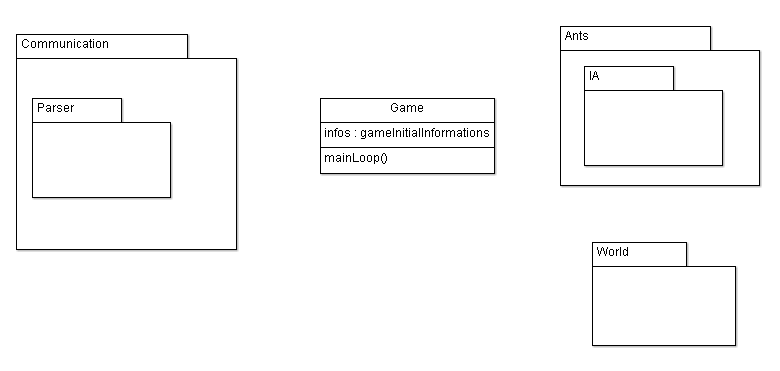
\includegraphics[width=\textwidth]{global.png}
  \caption{Architecture générale}
\end{figure}

\begin{figure}
  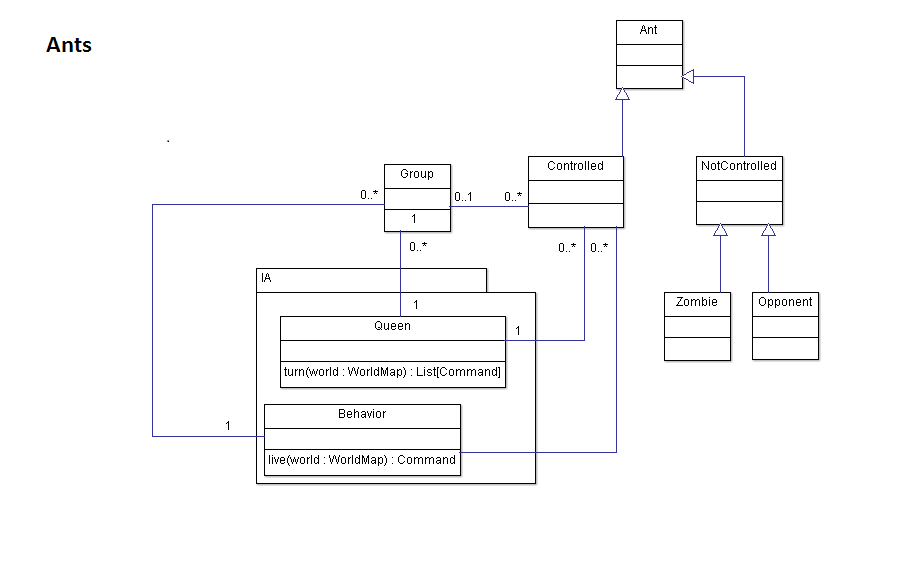
\includegraphics[width=\textwidth]{ants.png}
  \caption{Contenu du Package Ants}
\end{figure}

\begin{figure}
  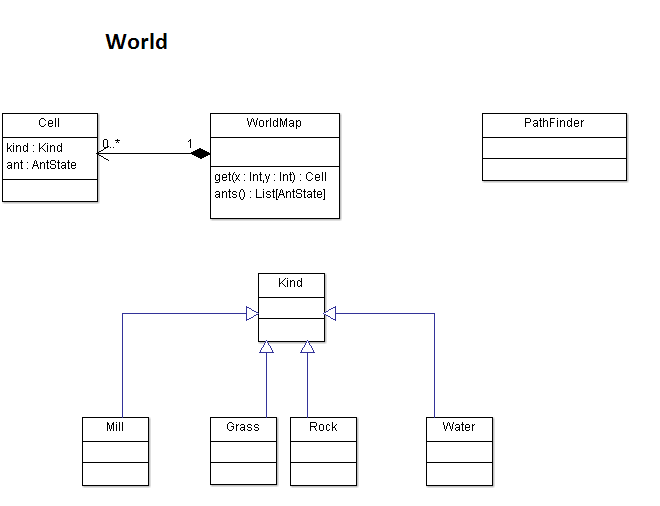
\includegraphics[width=\textwidth]{world.png}
  \caption{UML World}
\end{figure}

\begin{figure}
  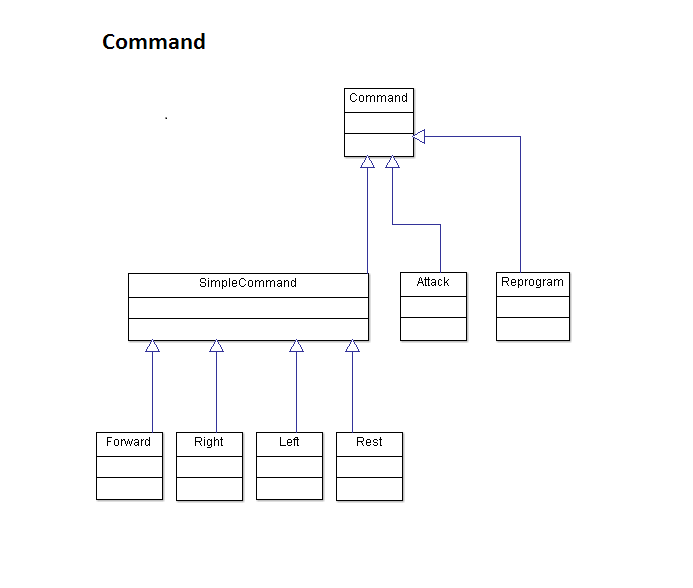
\includegraphics[width=\textwidth]{commands.png}
  \caption{UML Commandes}
\end{figure}

\end{document}